\documentclass{article}

\usepackage{graphicx}
\usepackage{tikz}
\usepackage{tikzsymbols}
\usetikzlibrary{calc,patterns,shapes.geometric}
\pagestyle{empty}
\usepackage[margin=0pt]{geometry}
\geometry{papersize={14in,12in}}

\def\centerarc[#1](#2)(#3:#4:#5){\draw[#1] ($(#2)+({#5*cos(#3)},{#5*sin(#3)})$) arc (#3:#4:#5);}

\begin{document}
	\begin{figure}
		\centering
		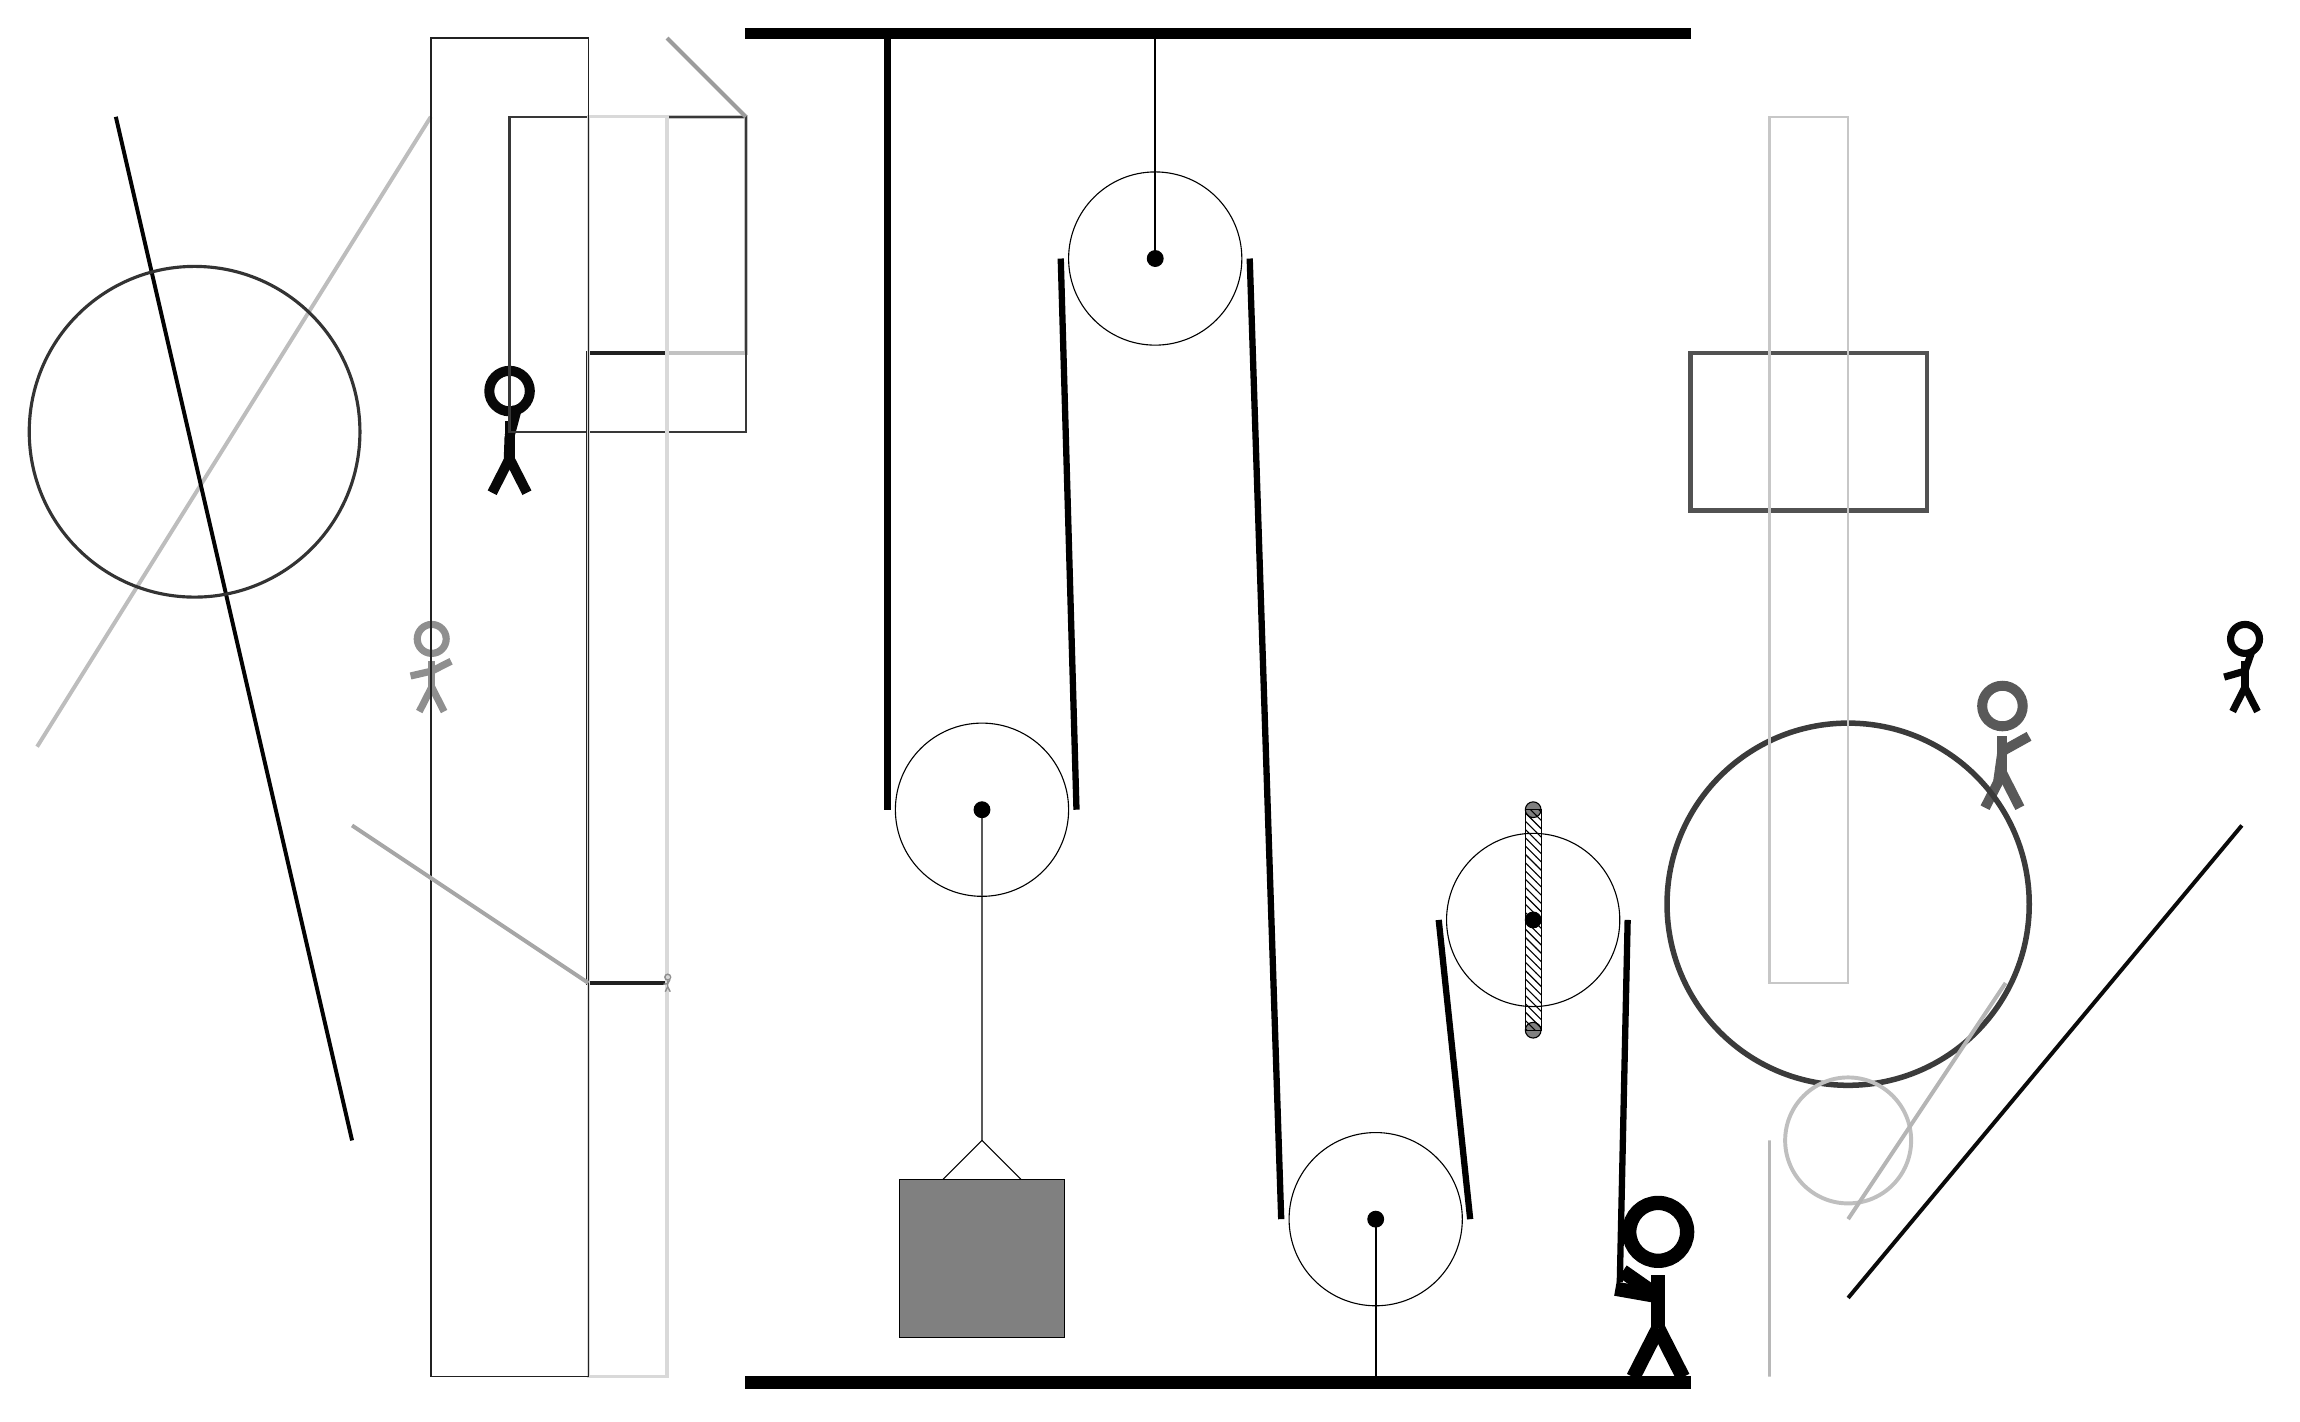
\begin{tikzpicture}
			%%%%% START %%%%%
			
			\draw[fill=black] (-2, 14) rectangle (10, 14.125);
			
			\draw (1, 4.2) circle (1.1);
			\draw[fill=black] (1, 4.2) circle (0.1);
			
			\draw (3.2, 11.2) circle (1.1);
			\draw[fill=black] (3.2, 11.2) circle (0.1);
			\draw[thick] (3.2, 11.2) -- (3.2, 14);
			
			\draw (6, -1) circle (1.1);
			\draw[fill=black] (6, -1) circle (0.1);
			\draw[thick] (6, -1) -- (6, -3);
			
			\draw[fill=white](8, 2.8) circle (1.1);
			\draw[fill=black] (8, 2.8) circle (0.1);
			\draw[fill=black!50] (8, 4.2) circle (0.1);
			\draw[fill=black!50] (8, 1.4) circle (0.1);
			\draw[pattern=north west lines, pattern color=black] (7.9, 4.2) rectangle (8.1, 1.4);
			
			\draw (1, 4.2) -- (1, 0) -- (0.5, -0.5);
			\draw (1, 0) -- (1.5, -0.5);
			\draw[fill=black!50] (-0.05, -0.5) rectangle (2.05, -2.5);
			
			\draw[line width=0.8mm] (-0.2, 14) -- (-0.2, 4.2);
			\centerarc[line width=0.8mm](1, 4.2)(180:360:1.2000000000000002);
			\draw[line width=0.8mm](2.2, 4.2) -- (2.0, 11.2);
			\centerarc[line width=0.8mm](3.2, 11.2)(0:180:1.2000000000000002);
			\draw[line width=0.8mm](4.4, 11.2) -- (4.8, -1);
			\centerarc[line width=0.8mm](6, -1)(180:360:1.2000000000000002);
			\draw[line width=0.8mm](7.2, -1) -- (6.8, 2.8);
			\centerarc[line width=0.8mm](8, 2.8)(0:180:1.2000000000000002);
			\draw[line width=0.8mm](9.2, 2.8) -- (9.1, -1.8);
			
			\node at (9.5, -1.9) {\Strichmaxerl[10][-35][170]};
			
			\draw[line width=0.5mm, color=black!49] (10, 1) rectangle (10, 1);
			
			\node[line width=0.6mm, color=black!97] at (-5, 9) {\Strichmaxerl[7][88][75]};
			\draw[line width=0.5mm, color=black!26](-6, 13) -- (-11, 5);
			\draw[line width=0.5mm, color=black!24] (-2, 13) rectangle (-3, 10);
			\node[line width=0.7mm, color=black!65] at (14, 5) {\Strichmaxerl[7][82][29]};
			\draw[line width=0.4mm, color=black!28] (11, -3) rectangle (11, 0);
			\node[line width=0.3mm, color=black!98] at (17, 6) {\Strichmaxerl[5][16][71]};
			
			\draw[line width=0.6mm, color=black!68] (10, 8) rectangle (13, 10);
			\draw[line width=0.3mm, color=black!78] (-2, 9) rectangle (-5, 13);
			\draw[line width=0.5mm, color=black!87] (-4, 10) rectangle (-3, 2);
			\draw [line width=0.7mm, color=black!77](12, 3) circle (2.3);
			
			\draw [line width=0.5mm, color=black!25](12, 0) circle (0.8);
			\draw[line width=0.4mm, color=black!15] (-4, 13) rectangle (-3, -3);
			
			\draw[line width=0.5mm, color=black!39](-3, 14) -- (-2, 13);
			\node[line width=0.3mm, color=black!44] at (-6, 6) {\Strichmaxerl[5][13][27]};
			\draw[line width=0.5mm, color=black!99](-7, 0) -- (-10, 13);
			
			\node[line width=0.7mm, color=black!44] at (-3, 2) {\Strichmaxerl[1][10][61]};
			
			\draw[line width=0.2mm, color=black!87] (-4, -3) rectangle (-6, 14);
			\draw[line width=0.5mm, color=black!29](14, 2) -- (12, -1);
			\draw[line width=0.3mm, color=black!22] (11, 2) rectangle (12, 13);
			\draw[line width=0.5mm, color=black!96](12, -2) -- (17, 4);
			\draw [line width=0.4mm, color=black!80](-9, 9) circle (2.1);
			
			\draw[line width=0.5mm, color=black!35](-7, 4) -- (-4, 2);
			
			\draw[fill=black] (-2, -3) rectangle (10, -3.15);
			
			%%%%% END %%%%%
		\end{tikzpicture}
	\end{figure}	
\end{document}